\documentclass[../thesis.tex]{subfiles}
\begin{document}
\chapter{Integrated Photoluminescence Lifetimes} \label{sec:integrated_lifetime}

\section{Luminance as Efficiency Loss}
\begin{equation}
\eta_{EQE}=\eta_{PL}\eta_{OC}\chi\eta_{EF}\eta_\tau
\label{eqn:eqe_quenching}
\end{equation}

\begin{equation}
\frac{\eta_{EQE}(t)}{\eta_{EQE}^0}=\frac{\eta_{PL}(t)}{\eta_{PL}^0}\frac{\eta_{EF}(t)}{\eta_{EF}^0}
\label{eqn_eqe_decay_components}
\end{equation}

\section{Photoluminescence Characterization}

\begin{equation}
\frac{\eta_{PL}(t)}{\eta_{PL}^0}=\frac{L_{PL}(t)}{L_{PL}^0}\frac{I^0}{I(t)}
\label{eqn:pl_decay}
\end{equation}

\begin{figure}[ht]
\centering
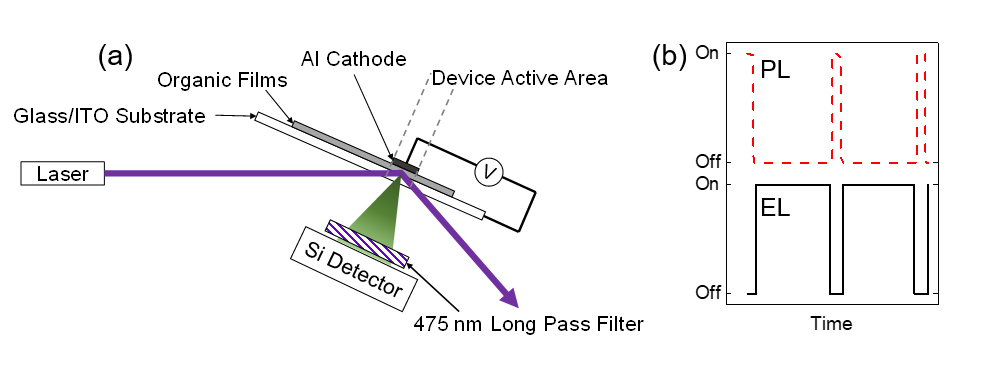
\includegraphics[width=0.48\textwidth]{integratedLifetime/schematic}
\caption{(a) Experimental configuration for the measurement of electro- (EL) and photoluminescence (PL) during OLED degradation.  Laser excitation is incident on a subsection of the device area.  The laser is aligned so that neither the incident nor reflected beam strikes the detector.  Stray laser light is removed by a $\lambda$=475 nm dielectric long pass filter.  (b) Excitation scheme.  EL and PL signals are probed independently with no temporal overlap.  (c) External quantum efficiency versus current density and luminance for devices having emissive layer thickness of 10 nm, 20 nm and 30 nm.}
\label{fig:schematic}
\end{figure}
\subsection{Light Selection}
\subsection{Absorption - Recombination Overlap}
\subsection{Contact Degradation}
\subsection{Quenching Changes During Degradation}
\begin{figure}[ht]
\centering
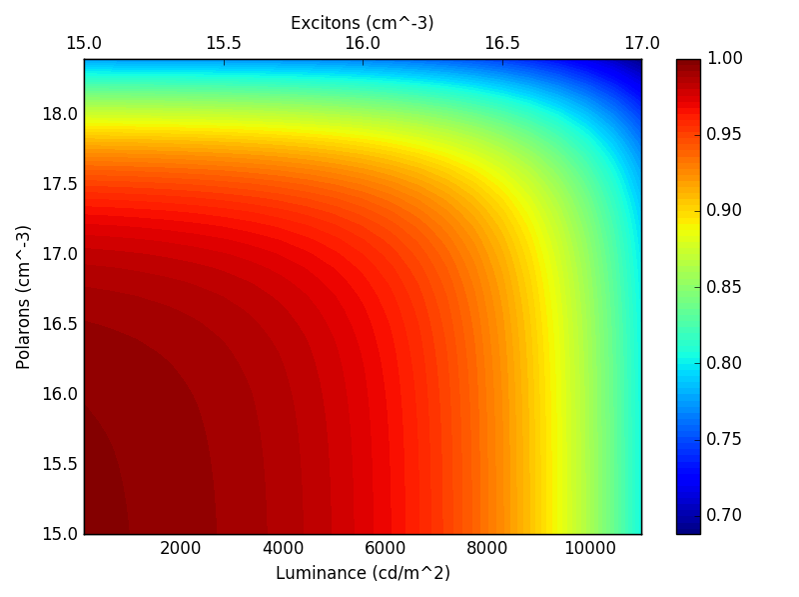
\includegraphics[width=0.48\textwidth]{integratedLifetime/quenching_correction}
\caption{Multiplicative correction factor for exciton formation efficiency due to changes in quenching during lifetime.  Shown as a function of polaron and exciton density as well as luminance, assuming a 10 nm emissive layer.}
\label{fig:quenching_correction}
\end{figure}
\subsection{Verification with Excton Lifetime}
\begin{figure}[ht]
\centering
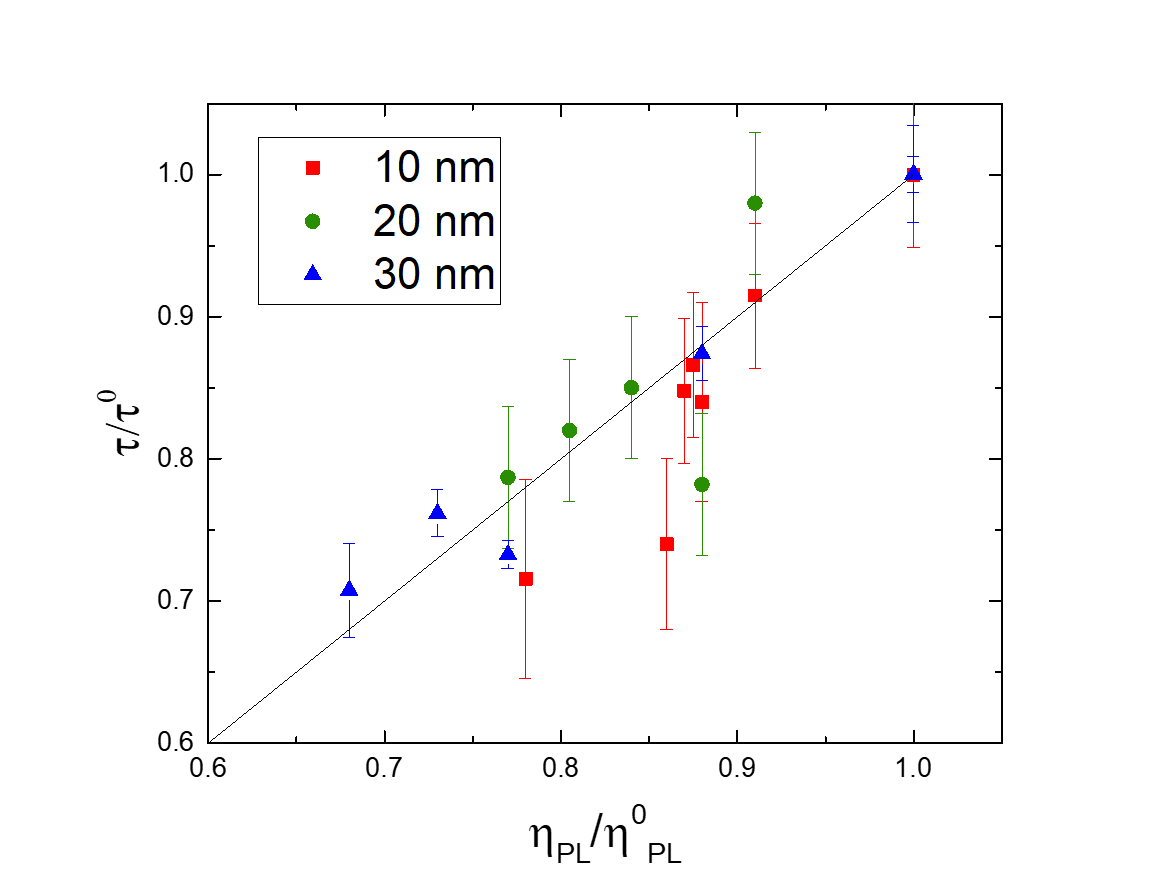
\includegraphics[width=0.48\textwidth]{integratedLifetime/transient_lifetimes}
\caption{Exciton lifetime ratio extracted from transient PL measurements on degraded and undegraded devices as a function of emissive layer thickness.}
\label{fig:transient_lifetimes}
\end{figure}

\section{Experimental Implementation}
\subsection{Hardware Setup}
\begin{figure}[ht]
\centering
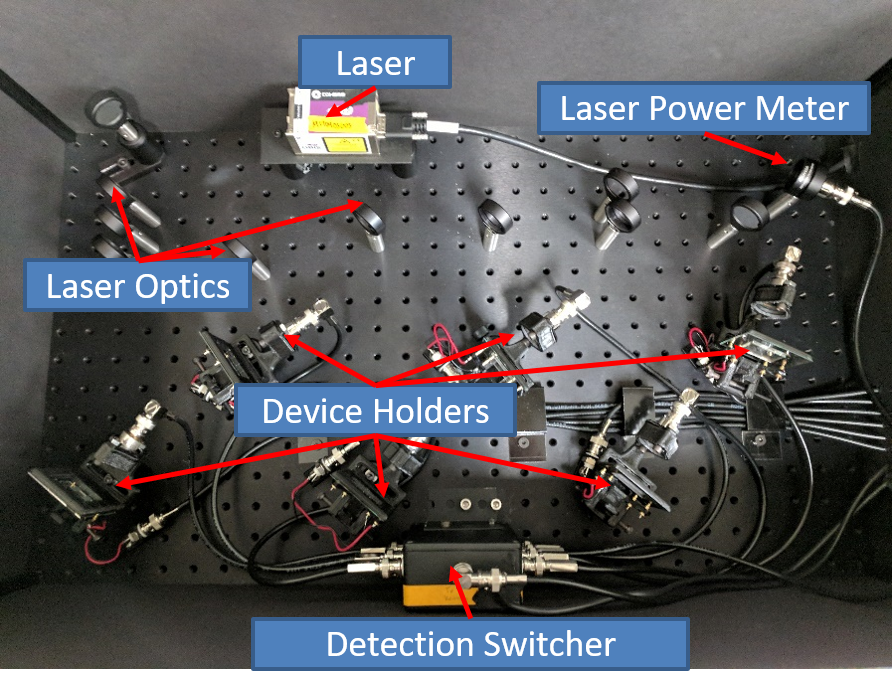
\includegraphics[width=0.48\textwidth]{integratedLifetime/hardware}
\caption{Device contacting, measurement, and optical hardware.  Version 3 of the hardware is shown.  Controlling hardware is shown in Fig. \ref{fig:source_measure}}
\label{fig:hardware}
\end{figure}

\begin{figure}[ht]
\centering
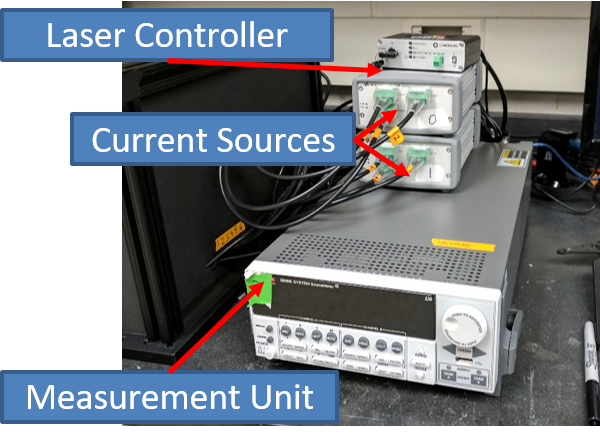
\includegraphics[width=0.48\textwidth]{integratedLifetime/source_measure}
\caption{Source-Measure hardware and laser controller}
\label{fig:source_measure}
\end{figure}

\subsection{Software Developement}

\begin{figure}[ht]
    \centering
    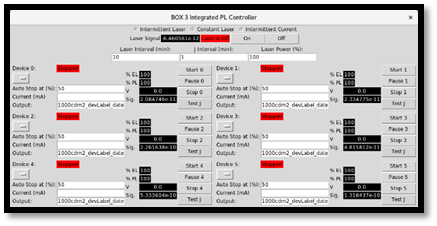
\includegraphics[width=0.48\textwidth]{integratedLifetime/software_controller}
\caption{6 channel software controller.  Selection of test type, laser control for allignment, and global settings are accessible on the top of the interface.  Individual channel settings are grouped on the bottom.}
\label{fig:software_controller}
\end{figure}

\subsection{Database Integration}
\begin{figure}[ht]
    \centering
    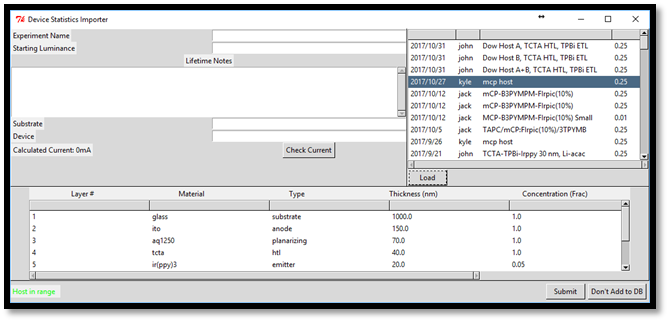
\includegraphics[width=0.48\textwidth]{integratedLifetime/lifetime_db_import}
\caption{Test information for database import interface.  The top left panel collects information about the specific device and lifetime.  The right panel connects the device to a particular growth and architecture.  The bottom panel confirms the architecture.}
\label{fig:lifetime_db_import}
\end{figure}


\ifcsdef{mainfile}{}{\bibliography{../library}}
\end{document}
